\documentclass[a4paper,10pt]{scrartcl}
\usepackage[utf8]{inputenc}
\usepackage{graphicx}
\usepackage{subfig}
\usepackage{amsmath}
\usepackage{geometry}
\geometry{a4paper,left=40mm,right=30mm, top=1cm, bottom=2cm} 
%opening
\title{TGI-1}
\author{}

\begin{document}
\section{Einführung in Begrifflichkeiten}

\subsection{Daten und Information}

\begin{itemize}
 \item \textbf{Defintion Information :} Information besitzt für den Empfänger einen Neugkeitsgehalt und 
 kann unterschiedlich übertragen werden
 \item \textbf{Daten} Repräsentieren Informationen (Bytefolge, Netzwerkpaket) $\Rightarrow$ Interpretation ergibt die Information
\end{itemize}


\subsection{Sicherheit}
\begin{itemize}
 \item \textbf{Definition Sicherheit: }Zustand oder subjektiver Eindruck frei von Gefahr
 \item \textbf{Definition Informationssicherheit: } Schutz der Information unabhängig von der Repräsentation 
 \item \textbf{IT-Sicherheit: }Schutz  
 \item \textbf{Zwei Formen der Sicherheit: } security (Angriff), safety(Betrieb)
\end{itemize}


\subsection{Kommunikationskanäle}

\begin{itemize}
 \item \textbf{Kommunikation: }Nachrichtenaustausch zwischen mindestens zwei Partnern oder Gegenstellen
 \item \textbf{Kommunikationskanal: } Notwendig für den Informationsfluss zwischen Sender und Empfänger
 \item \textbf{Legitime Kanäle: } Vorgesehen für den Informationsaustausch z.B Sprache über Telefon
 \item \textbf{Verdeckte Kanäle: } Kanal der absichtlich aber unabsichtlich zur Kommunikation missbraucht wird. Z.B. versteckte 
 Botschaften in Bildern (Stenographie)
\end{itemize}


\subsection{Bedrohung}

\begin{itemize}
 \item \textbf{Gefährdungsfaktoren nach BSI := Bundesamt für Sicherheit in der Informationstechnik: } 
 Höhere Gewalt, Vorsätzliche Handlung, Technische Fehler, Fahrlässigkeit, Organisatorische Mängel
\item \textbf{Verwundbarkeit: }Schwachstelle beziehungsweise eine Sicherheitslücke des Systems,
mittels derer die vorhandenen Sicherheitsmechanismen umgangen oder
getäuscht werden können.
\item \textbf{Bedrohung: } Ereignis aus dem Schaden entstehen kann.
\end{itemize}

\subsection{Angriff}

\begin{itemize}
 \item \textbf{Angriff: } bezeichnet einen nicht autorisierten Zugriff(sversuch) auf ein It-Sytem oder Information.
 \item \textbf{aktiver Angriff: } nicht autorisierte Informationsveränderung, richtet sich typischerweise gegen die Integrität oder
Verfügbarkeit des Systems
\item \textbf{passiver Angriff: } nicht autorisierten Informationsgewinne: zuschauen, mithören, aufzeichnen
\end{itemize}

\subsection{Risiko}

\begin{itemize}
 \item \textbf{Risiko}  Risiko = Eintrittswahrscheinlichkeit * Schadenshöhe
\end{itemize}

\subsection{Schutzziele}

\begin{itemize}
 \item \textbf{Schutzziel} Ziel der Sicherheitsmaßnahmen, um
ein System gegen bestimmte Angriffe zu schützen 
 \item \textbf{Vertraulichkeit}  Informationen nur für diejenigen Personen oder
Ressourcen zugänglich sind, welche für einen Zugriff berechtigt sind (Zugriffskontrolle, Verbergen der Information( Stenographie), Verschlüsselung)
 \item \textbf{Integrität} Unversertheit der Daten (Zugriffskontrolle, elektronische Signatur)
 \item \textbf{Authentizität} Authentizität bedeutet, dass der Urheber einer
Information bekannt ist (Authentizitätsverfahren)
 \item \textbf{Zurechenbarkeit} beschreibt die Eigenschaft, dass es nicht möglich ist,
eine Aktion gegenüber unbeteiligten Dritten
abzustreiten. (Sicherstellen über Integrität und Authentizität)
 \item \textbf{Verfügbarkeit} bedeute das es autorisierten Subjekt möglich ist, die
Funktionalität der Ressource zu nutzen, wenn diese
benötigt wird (Sicherstellen durch reduntante Systeme) 
\end{itemize}

\subsection{Anonymisierung und Pseudonymisierung}
\begin{itemize}
\item \textbf{Anonymität}beschreibt die Eigenschaft, dass es nicht
oder nur mit unverhältnismäßig großem Aufwand
möglich ist, die Identität eines Subjekts zu bestimmen. (Stärker als Pseudonymisierung)(nur möglich bei großer Menge Individuen)
\item \textbf{Pseudonymität} hingegen versteht man das Verändern
einer Identität anhand einer Zuordnungsvorschrift, die
die echte Identität auf ein zugehöriges Pseudonym
abbildet. Kommunikationspartner sehen nur das
Pseudonym.
\end{itemize}
\subsection{Zussammenfassung}

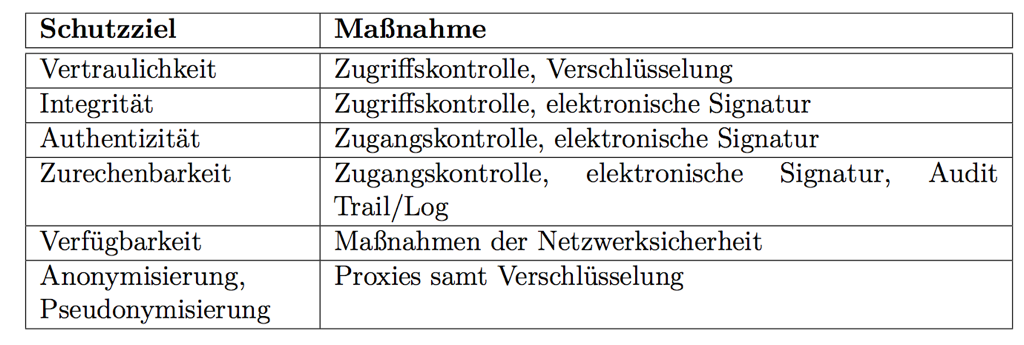
\includegraphics[width =\textwidth]{test.png}

Proxies weil sie andere IP zur Verfügung stellen - deswegen gut für Pseudonymisierung geeignet


\end{document}